% Copyright 2006 by Till Tantau
%
% This file may be distributed and/or modified
%
% 1. under the LaTeX Project Public License and/or
% 2. under the GNU Free Documentation License.
%
% See the file doc/generic/pgf/licenses/LICENSE for more details.


\section{Tree Library}
\label{section-tree-library}

\begin{tikzlibrary}{trees}
    This packages defines styles to be used when drawing trees.
\end{tikzlibrary}
%
\begin{codeexample}[setup code,hidden]
    \usetikzlibrary{trees}
\end{codeexample}


\subsection{Growth Functions}

The package |trees| defines two new growth functions. They are installed using
the following options:

\begin{key}{/tikz/grow via three points=\texttt{one child at (}\meta{x}
        \texttt{) and two children at (}\meta{y}\texttt{) and (}\meta{z}|)|%
}
    This option installs a growth function that works as follows: If a parent
    node has just one child, this child is placed at \meta{x}. If the parent
    node has two children, these are placed at \meta{y} and \meta{z}. If the
    parent node has more than two children, the children are placed at points
    that are linearly extrapolated from the three points \meta{x}, \meta{y},
    and \meta{z}. In detail, the position is $x + \frac{n-1}{2}(y-x) +
    (c-1)(z-y)$, where $n$ is the number of children and $c$ is the number of
    the current child (starting with~$1$).

    The net effect of all this is that if you have a certain ``linear
    arrangement'' in mind and use this option to specify the placement of a
    single child and of two children, then any number of children will be
    placed correctly.

    Here are some arrangements based on this growth function. We start with a
    simple ``above'' arrangement:
    %
\begin{codeexample}[]
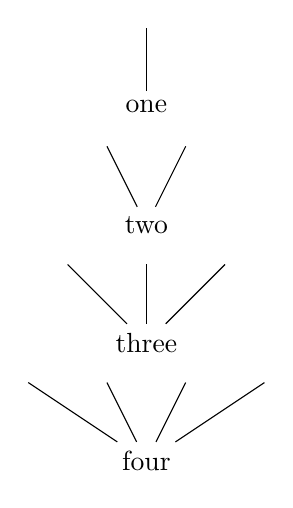
\begin{tikzpicture}[grow via three points={%
    one child at (0,1) and two children at (-.5,1) and (.5,1)}]
  \node at (0,0) {one} child;
  \node at (0,-1.5) {two} child child;
  \node at (0,-3) {three} child child child;
  \node at (0,-4.5) {four} child child child child;
\end{tikzpicture}
\end{codeexample}

    The next arrangement places children above, but ``grows only to the
    right''.
    %
\begin{codeexample}[]
\begin{tikzpicture}[grow via three points={%
    one child at (0,1) and two children at (0,1) and (1,1)}]
  \node at (0,0) {one} child;
  \node at (0,-1.5) {two} child child;
  \node at (0,-3) {three} child child child;
  \node at (0,-4.5) {four} child child child child;
\end{tikzpicture}
\end{codeexample}

    In the final arrangement, the children are placed along a line going down
    and right.
\begin{codeexample}[]
\begin{tikzpicture}[grow via three points={%
    one child at (-1,-.5) and two children at (-1,-.5) and (0,-.75)}]
  \node at (0,0) {one} child;
  \node at (0,-1.5) {two} child child;
  \node at (0,-3) {three} child child child;
  \node at (0,-4.5) {four} child child child child;
\end{tikzpicture}
\end{codeexample}

    These examples should make it clear how you can create new styles to
    arrange your children along a line.
\end{key}

\begin{key}{/tikz/grow cyclic}
    This style causes the children to be arranged ``on a circle''. For this,
    the children are placed at distance |\tikzleveldistance| from the parent
    node, but not on a straight line, but on points on a circle. Instead of a
    sibling distance, there is a |sibling angle| that denotes the angle between
    two given children.
    %
    \begin{key}{/tikz/sibling angle=\meta{angle}}
        Sets the angle between siblings in the |grow cyclic| style.
    \end{key}
    %
    Note that this function will rotate the coordinate system of the children
    to ensure that the grandchildren will grow in the right direction.
    %
\begin{codeexample}[]
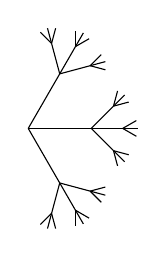
\begin{tikzpicture}
  [grow cyclic,
   level 1/.style={level distance=8mm,sibling angle=60},
   level 2/.style={level distance=4mm,sibling angle=45},
   level 3/.style={level distance=2mm,sibling angle=30}]
  \coordinate [rotate=-90] % going down
    child foreach \x in {1,2,3}
      {child foreach \x in {1,2,3}
        {child foreach \x in {1,2,3}}};
\end{tikzpicture}
\end{codeexample}
    %
\end{key}

\begin{key}{/tikz/clockwise from=\meta{angle}}
    This option also causes children to be arranged on a circle. However, the
    rule for placing children is simpler than with the |grow cyclic| style: The
    first child is placed at \meta{angle} at a distance of
    |\tikzleveldistance|. The second child is placed at the same distance from
    the parent, but at angle \meta{angle}${}-{}$|\tikzsiblingangle|. The third
    child is displaced by another |\tikzsiblingangle| in a clockwise fashion,
    and so on.

    Note that this function will not rotate the coordinate system.
    %
\begin{codeexample}[]
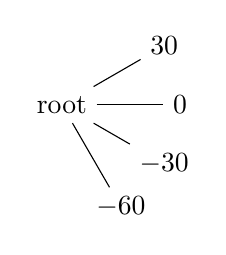
\begin{tikzpicture}
  \node {root}
  [clockwise from=30,sibling angle=30]
  child {node {$30$}}
  child {node {$0$}}
  child {node {$-30$}}
  child {node {$-60$}};
\end{tikzpicture}
\end{codeexample}
    %
\end{key}

\begin{key}{/tikz/counterclockwise from=\meta{angle}}
    Works the same way as |clockwise from|, but sibling angles are added
    instead of subtracted.
\end{key}


\subsection{Edges From Parent}

The following styles can be used to modify how the edges from parents are
drawn:

\begin{stylekey}{/tikz/edge from parent fork down}
    This style will draw a line from the parent downwards (for half the level
    distance) and then on to the child using only horizontal and vertical
    lines.
    %
\begin{codeexample}[]
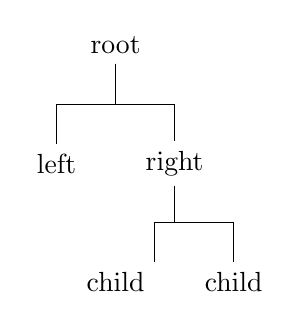
\begin{tikzpicture}
  \node {root}
    [edge from parent fork down]
    child {node {left}}
    child {node {right}
      child[child anchor=north east] {node {child}}
      child {node {child}}
    };
\end{tikzpicture}
\end{codeexample}
    %
\end{stylekey}

\begin{stylekey}{/tikz/edge from parent fork right}
    This style behaves similarly, only it will first draw its edge to the
    right.
    %
\begin{codeexample}[]
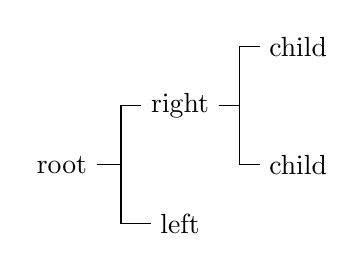
\begin{tikzpicture}
  \node {root}
    [edge from parent fork right,grow=right]
    child {node {left}}
    child {node {right}
      child {node {child}}
      child {node {child}}
    };
\end{tikzpicture}
\end{codeexample}
    %
\end{stylekey}

\begin{stylekey}{/tikz/edge from parent fork left}
    Behaves similarly to the previous styles.
\end{stylekey}

\begin{stylekey}{/tikz/edge from parent fork up}
    Behaves similarly to the previous styles.
\end{stylekey}


%%% Local Variables:
%%% mode: latex
%%% TeX-master: "pgfmanual-pdftex-version"
%%% End:
